
%%%%%%%%%%%%%%%%%%%%%%% file typeinst.tex %%%%%%%%%%%%%%%%%%%%%%%%%
%
% This is the LaTeX source for the instructions to authors using
% the LaTeX document class 'llncs.cls' for contributions to
% the Lecture Notes in Computer Sciences series.
% http://www.springer.com/lncs       Springer Heidelberg 2006/05/04
%
% It may be used as a template for your own input - copy it
% to a new file with a new name and use it as the basis
% for your article.
%
% NB: the document class 'llncs' has its own and detailed documentation, see
% ftp://ftp.springer.de/data/pubftp/pub/tex/latex/llncs/latex2e/llncsdoc.pdf
%
%%%%%%%%%%%%%%%%%%%%%%%%%%%%%%%%%%%%%%%%%%%%%%%%%%%%%%%%%%%%%%%%%%%


%\documentclass[runningheads]{llncs}
\documentclass{llncs}

\usepackage[utf8]{inputenc}
\usepackage[T1]{fontenc}
\usepackage{lmodern}

\usepackage{amssymb}
\usepackage{url}
\setcounter{tocdepth}{3}
\usepackage{graphicx}
\usepackage{mfirstuc}
\usepackage{url}
\urldef{\mailsa}\path|{diego}@geutstudio.com|
\newcommand{\keywords}[1]{\par\addvspace\baselineskip
\noindent\keywordname\enspace\ignorespaces#1}

\RequirePackage[
  colorlinks,
  citecolor=red,
  linkcolor=blue,
  menucolor=blue,
  %urlcolor=blue, % use hyperref defaults
  linktocpage,
  naturalnames,
  plainpages,
  final
]{hyperref}

\hypersetup{
  % Your metadata go here
  pdftitle={Technical Draft: A platform to augment web applications with multimodal interactions},
  pdfauthor={Diego Paez},  
  pdfkeywords={Multimodal Interaction, Web Applications, Platform, Mobile Interaction Design},
  pdfsubject={Multimodal Interaction}
}

\begin{document}
\mainmatter  % start of an individual contribution

% first the title is needed
\title{\capitalisewords{A platform to augment web applications with multimodal interactions}}
\subtitle{\textbf{Technical Draft}}

% a short form should be given in case it is too long for the running head
%\titlerunning{Lecture Notes in Computer Science: Authors' Instructions}

% the name(s) of the author(s) follow(s) next
%
% NB: Chinese authors should write their first names(s) in front of
% their surnames. This ensures that the names appear correctly in
% the running heads and the author index.
%
\author{Diego Paez}
%
\authorrunning{Technical Draft: A platform to augment web applications with multimodal interactions}
% (feature abused for this document to repeat the title also on left hand pages)

% the affiliations are given next; don't give your e-mail address
% unless you accept that it will be published
\institute{Geut Labs\\
1900 La Plata, Argentina\\
\mailsa\\
\url{http://geutstudio.com/}}

%
% NB: a more complex sample for affiliations and the mapping to the
% corresponding authors can be found in the file "llncs.dem"
% (search for the string "\mainmatter" where a contribution starts).
% "llncs.dem" accompanies the document class "llncs.cls".
%

\toctitle{Lecture Notes in Computer Science}
\tocauthor{Authors' Instructions}
\maketitle


\begin{abstract}
Here we are introducing a novel platform that expands, what we called, the common set of interactions on web applications. Further more, this platform not only helps to increase this set, but also adds multimodal interactions capabilities to web applications. The way the multimodal interaction is supported is based on a different approach introduced here as a distributed fusion system.
\end{abstract}

% =============================================================================
\section{Introduction}
% =============================================================================
Web Applications are increasingly popular. A huge number of people access to applications from anywhere using new devices that have potential for different forms of interaction. Web applications designers, developers and modality engineers are faced everyday with the need to support these new interactions in their products.

We propose a platform that helps a multimodal development team to add new modalities in the context of a web application. This modalities can work standalone or together generating a multimodal experience. 

This platform helps to increase the set of interactions to be supported (beyond the usual modalities found on desktop computers and mobile devices) including: keyboard, mouse, optic (pens), haptics (i.e touch devices, vibro-tactile feedback) and gestures (e.g Microsoft Kinect or Leap Motion). Whilst this set offers a good amount of interaction capabilities, it is extremely rare to found all of these together on ``a single device'', further more to found applications that uses all or even some of them, gives scarce results. 

With the proposed platform, we can ``integrate'' different modalities found on different devices, inside the context of a Web application and distribute the interaction. 

We have a simple working demo using two different modalities, haptics and air gestures, and they can be seen as two separate modalities or as a single multimodal interaction.

% =============================================================================
\section{Related Work}
% =============================================================================
There are not many contemporary works that addressed the main subject of this paper, add support for multimodal interactions on web applications. However, some interesting and similar solutions can be cited:
\begin{enumerate}

\item i*Chameleon \cite{lo2013chameleon}, introduces an MVC framework for developing multimodal applications. They combine the \emph{separation of responsibilities} principle with all the different roles involved on the development of a multimodal application. This results in a ``easy to follow'' workflow which was an inspiration for our work. A key difference with our solution is the fact that i*Chameleon is a framework and we propose a platform (i.e the \emph{Plusultra} instances allows to handle multiple web applications, not just multiple clients). According to the nature of Web applications, we needed to add an extra service layer in order to being capable of have a multimodal channel open per client.

\item Multimodal Framework for Mobile Interaction \cite{cutugno2012multimodal}, on this work they target mobile because these devices offer a rich set of sensors and actuators and they are very popular, we share this vision but we try to integrate every device capable of access the web, not only mobile. Another important aspect of this work it is they follow the W3C guides \cite{w3c:mmiframework} \cite{w3c:mmiarch}. But then they validate their work developing a native application (Android). We took some design characteristics of the architecture proposed by the W3C, but or work is not fully compliant with their guidelines.

\item Mudra \cite{Hoste2011}, introduces a unified multimodal framework. We found many similarities on the design ideas. While \emph{Plusultra} can be classified as a data stream oriented architecture, there is a possibility to add more data processing stages as filters connected with the modality drivers output or as pre-processing input at the \emph{Plusultra}'s entrance. Multiple users support and collaboration are features that are present on \emph{Plusultra} and are almost transparent for the developer. These features were added with no cost thanks to capabilities inherent to Web applications.
\end{enumerate}

% =============================================================================
\section{The Platform}
% =============================================================================
The platform architecture is composed by two separate parts, a distributed publisher/subscriber system, named \emph{Plusultra}, and an endpoint dependency, known as \emph{Gyes}. They ``talk'' each other using a top-level protocol specifically designed for the platform. Figure \ref{fig:arq_simple} shows these components. 

Circles represent a \emph{Plusultra} instance, working as a message gateway, surrounding it are the Web clients and one or more modality devices. They are using the component \emph{Gyes} to connect with the system and exchange modality information. 

\begin{figure}
  \centering
  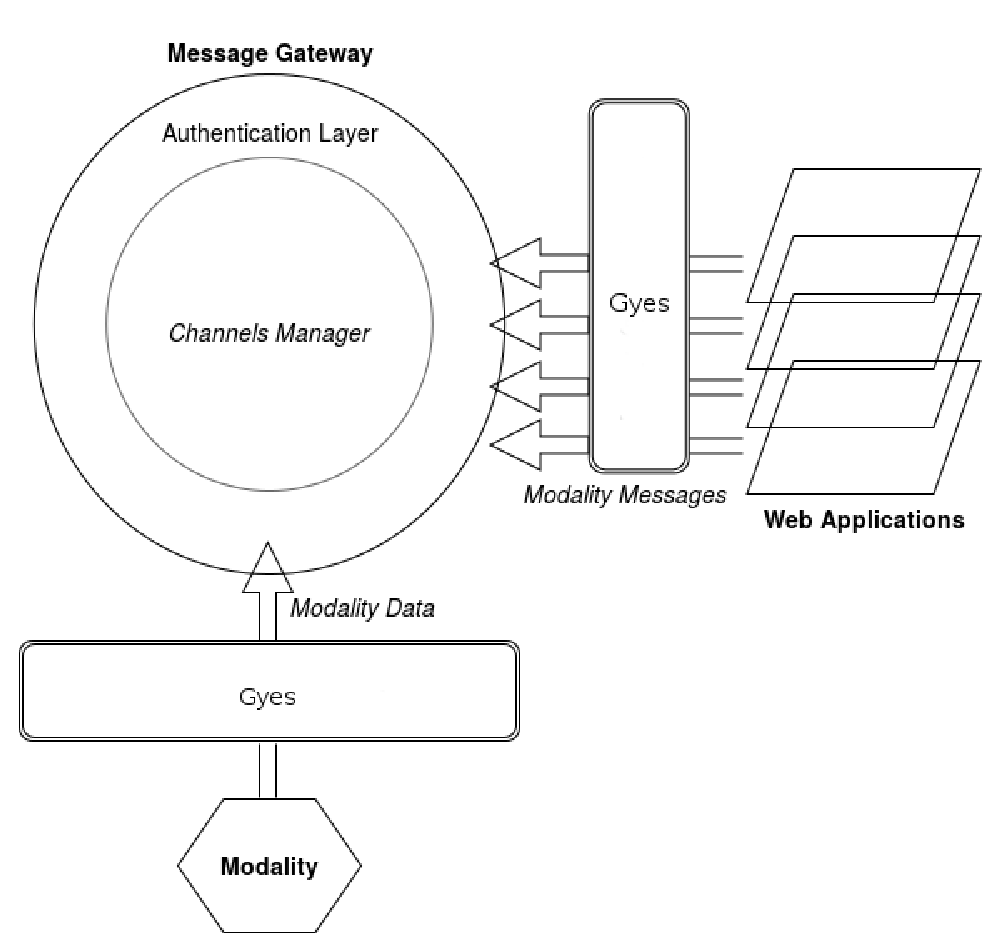
\includegraphics[height=7.5cm]{arq_simple_bw.eps}
  \caption{A quick view of the platform.}
  \label{fig:arq_simple}
\end{figure}


The following sub-sections will provide more information about each single part of the platform.

\subsection{Communication: Plusultra}

The communication component consists on a Node.js \cite{ind:nodejs} real-time service. It handles messages from web clients and modality devices and using an in-memory storage can quickly distribute them between all the connected parts. It provides a websocket server on which \emph{Gyes} modules can connect.

Every service instance works like a distributed publishers/subscribers system, so it can escalate horizontally easily~\cite{Kermarrec2003}. More instances can be instantiated, having each of these a CPU core assigned, then they can be connected to the in-memory storage in order to have a common place to store and get dynamic information from connected modalities and clients.

The system is based on events and it works in a reactive way. This decision was based considering the modalities nature. They are usually recognizers devices that can originate bursts of data which are triggered as events and propagated using the \emph{Plusultra} component.
Using a communication paradigm like this give us a clear separation between modalities and web clients~\cite{Kermarrec2003}.

\subsection{Modalities and Web Applications: Gyes}

The endpoint component \emph{Gyes}, can run on the client side and on modality devices too. It is mainly used by the Web Developer, the Device Engineer and possibly the Modality Designer. It is consumed like another dependency on the development stack and in general terms, it allows to connect with the \emph{Plusultra} component, add new modalities to a web application, propagate data recognized by modalities and act, synthesizing data if possible. 

Like we mentioned before, this same component can run on Modality Devices too. When it is used like this, it becomes a \emph{Modality Driver}. It enables the Modality Engineer to connect a new modality with the platform and it is the point where recognizer's events are defined and/or what type of fission can handle the device. On the next listing we can see a Modality Driver Interface's sample:
\noindent
\begin{verbatim}
var ModalityDriverChannel = require( 'gyes' ).ModalityDriver; 

function HapticModalityDriver( opts ){
    // initialization code...
	
    // This driver can run on a variety of devices. 
    // It is important to check if the device can perform 
    // the desired fission action. 
    if ( this.vibrate ){
        this.on( 'synthetized', this.fission.bind(this) );
    }
}

inherits( HapticModalityDriver, ModalityDriverChannel );

HapticModalityDriver.prototype.fission = function( time ){
    time = time || 1000;
    var pattern = [];
    pattern.push( time );
    this.vibrate( pattern );
};
\end{verbatim}
\noindent
{\small Using Gyes to create a Modality Driver Node.js hybrid module.} 

\subsection{Interpretations}
We use a concept similar to the ``Facts'' introduced with Mudra \cite{Hoste2011}. The term we use is \emph{interpretations} and they define a semantic structure which works primarily as an events set.
 
These events can be originated from applications or via modalities. An interpretation is said to ``happen'' when all of their events are detected inside a defined time span (they have been originated elsewhere and transmitted through the platform). The detection logic is managed by the Gyes component, specifically by the Fusion engine.
 
But interpretations are not only events containers, they can be used to define a ``synthesize'' action, i.e., if a modality driver can synthesize, an interpretation can be attached to this action and then when the interpretation happens, the action will be executed on every client capable of handle it.

Interpretations are used as the main input of the system. In order to be detected, an interpretation structure must be delivered to the Fusion engine \emph{fuse} action.
On the other side, the Fission engine can be used to attach custom actions to interpretations. These actions will be executed when a particular interpretation occurs, i.e., when a fission event is detected.
%Below, there is a code snippet showing the interpretation creation:
%\noindent
%\begin{verbatim}
%// Creation, using the gyes component.
%_gestureInterpretation = new gyes.Interpretation( [’fingerover’, 
%’hold’] );
%// Setting up an interpretation synthesize.
%_gestureInterpretation.canSynthetize( hapticMod.name, 
%hapticDriver.getID(), 2000 );
%\end{verbatim}
%\noindent
%{\small A Gyes interpretation.} 
\subsection{Distributed Fusion \& Fission Engines}
The architecture proposed here, follows the one introduced by Dumas et al. \cite{Dumas2009}. Since this module works on the client, we decided to move most of the Integration Committee inside of it, making it directly available to the developer. This decision goes hand-in-hand with the web application development style, having a heavy client with more logic on it side, in order to improve user interaction~\cite{Fraternali2010a}. This also means that the Fusion and Fission engines are distributed on every Web application client.

The main responsibility of the Fusion system is to fuse interactions, listening for events. When a interaction happens, a message is send to \emph{Plusultra} to be broadcasted to all others clients. This action will originate multiple fissions, which can led to multiple synthesis event. 

\subsection{Overview}
These proposed architecture works similar to the heartbeat parallel architecture, i.e. recognizers can be distributed along and within web clients, when an interpretation is found, this means that the fusion engine has detected it and the following actions will be to activate the fission engine. This is where the Web Developer can add custom business logic. This mechanism happens on a single web client and it is distributed along the others clients connected to the platform. 
The following figure \ref{fig:shapes_arq_simple} summarizes \emph{Plusultra} and \emph{Gyes} usage on a sample application called ``shapes''.

\begin{figure}
	\centering
	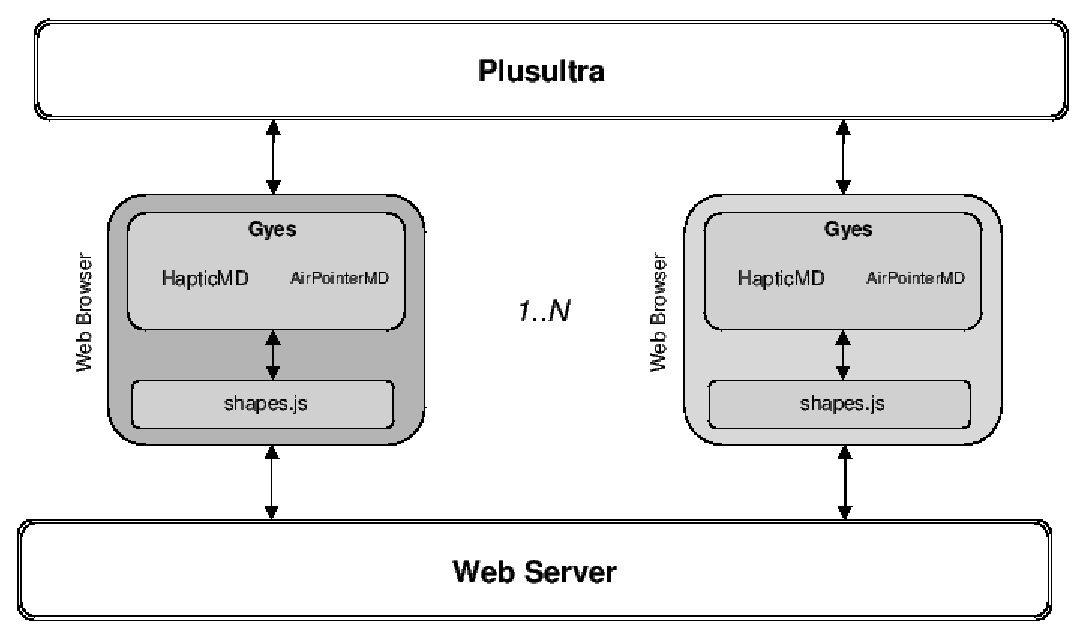
\includegraphics[height=6cm]{shapes_app_arq_en_bw.eps}
	\caption{Multiple Gyes modules interacting with the Plusultra platform.}
	\label{fig:shapes_arq_simple}
\end{figure}

Shapes was developed like a proof of concept application, the main objective is to move letters to their respective containers, similar to shapes game that little kids used to play. The applications works in a collaborative way. One user can interact using air gestures, pointing a finger to a letter and moving it to the container, when is on top of the correct container (same shape), another user can ``push it'' inside. This is done using a tactile interaction through a smart phone, performing a \emph{hold} gesture over the container. 
This unlocks a simple visual effect and triggers the whole Fusion and Fission engines, dispatching a Fission output manifested as a vibration on every device capable, usually smart phones and some tablets devices.
%Shapes figures here

\section{Conclusions \& Further Work}
The platform introduced here allows to augment web applications with multimodal interactions. Also, the proposed architecture introduces a novel approach distributing the fusion and fission engines along the clients. 
Using this platform, Web developers can consume modality data and use it in the context of a web application and Device Engineers have a way to extend \emph{Gyes} in order to connect new modalities. 

It remains as future work to keep using the platform, improving it's interface, in order to make more easy the creation of web applications with multimodal interactions. It is also interesting to explore the possibility to develop a catalog of modality drivers, since we have seen it is easy to develop re-usable drivers using the current \emph{Gyes} interface.

\section{Acknowledgments}
I would like to thanks to my partner from \textbf{GeutStudio} ~\& \textbf{GeutLabs}, Martin Acosta, for his helpful feedback and his solid collaboration on the upcoming demo application.

\bibliographystyle{plain}
\bibliography{technical_draft_plusultra}
\end{document}

